% % !TeX program = xelatex
% !TeX spellcheck = es_ES
% !TeX encoding = utf8

\documentclass[onecolumn,10pt,titlepage,a4paper]{article}

\usepackage[a4paper,top=2.5cm,bottom=2cm,left=2cm,right=2cm,marginparwidth=1.75cm,headheight=28pt]{geometry}
% Formateo para castellano
%\usepackage[utf8]{inputenc}
\usepackage[spanish,mexico]{babel}
%\usepackage{natbib}



%Bibliografía

% Simbolos para notas de pie
\usepackage[symbol]{footmisc}
\renewcommand*{\thefootnote}{\fnsymbol{footnote}}

% \renewcommand{\thefootnote}{\fnsymbol{footnote}}
% \footnote[num]{text}

% \pagestyle{myheading}
% \markright{Mi Documento \hfill Mi nombre \hfi}
%
\usepackage{fancyhdr,framed}
\setlength{\headheight}{15.2pt}
\pagestyle{fancy}
\lhead{Elementos Finitos II - 31.92 \\ Patricio Whittingslow -- 55423}
\chead{TP 2}


%\usepackage{subcaption}

% Para el entorno align


% Multiples columnas para glosario
\usepackage{multicol}

%Figuras y subtitulos
\usepackage{graphicx}
\usepackage{caption,subcaption}
\usepackage{hyperref}
\hypersetup{
    colorlinks,
    citecolor=black,
    filecolor=black,
    linkcolor=black,
    urlcolor=black
}
\usepackage[utopia,expert]{mathdesign} %Opcion "expert" para no romperme las smallcaps de helvetica. 
\usepackage{amsmath}

\newcommand{\rmfont}[1]{{\fontfamily{ptm}\selectfont%
		#1}}
\newcommand{\rmfontbf}[1]{{\fontfamily{ptm}\selectfont%
		\textbf{#1}}}
\newcommand{\rmfontsc}[1]{{\fontfamily{ptm}\selectfont%
		\textsc{#1}}}
    
\newcommand{\Matlab}{\rmfont{\sc Matlab}}
    \newcommand{\Adina}{{\sc ADINA}}
    \newcommand{\refp}[1]{(\ref{#1})}
    \newcommand{\unspace}{\!\!\!\!\!\!\!\!\!\!\!\!\!\!\!\!\!\!\!\!}
    \newcommand{\ms}{\ \ \ } %Matrix Spacing
    \newcommand{\di}{\textrm{d}}
    \newcommand{\jac}{\rmfontbf{J}}
    \newcommand{\Djac}{|\;\jac\;|}
    \newcommand{\dNi}{\di N_i}
    \newcommand{\sigmab}{\boldsymbol{\sigma}}
    \newcommand{\varepsilonb}{\boldsymbol{\varepsilon}}
    \newcommand{\Phib}{\boldsymbol{\Phi}}
    \newcommand{\CPhi}{\boldsymbol{\{ } \Phi \boldsymbol{\} }}
    \newcommand{\Mme}[1]{\boldsymbol{[}\mathbf{#1} \boldsymbol{]}}
    \newcommand{\Rme}[1]{\boldsymbol{\lfloor}\mathbf{#1} \boldsymbol{\rfloor}}
    \newcommand{\Cme}[1]{\boldsymbol{\{ }\mathbf{#1} \boldsymbol{\}} }
    \newcommand{\MB}{\Mme{B}}
    \newcommand{\MN}{\Mme{N}}
    \newcommand{\ME}{\Mme{E}}
    \newcommand{\Mk}{\Mme{k}}
    \newcommand{\MA}{\Mme{A}}
    \newcommand{\radial}{r}
    \newcommand{\eff}{f}
%Helvetica
\renewcommand{\familydefault}{\sfdefault}
\usepackage[scaled=1]{helvet}
\usepackage[format=plain,
            labelfont={bf,it},
            textfont=it]{caption}
%\usepackage[T1]{fontenc}
%--------------------------------------


\usepackage{siunitx}
\newcommand{\glossentry}[2]{$#1\ $ \indent #2 \par \vspace{.4cm} }
\newcommand{\adm}{\textrm{adm}}


\title{Informe Técnico - ITBA}

\author{Patricio Whittingslow}
%========================> Comienza Documento
\begin{document}
\begin{titlepage}
	\centering
	
	{ \large Instituto Tecnológico de Buenos Aires  \par }
	\vspace{2cm}
	{\Large \scshape Elementos Finitos II - 31.92 \par}
	\vspace{2cm}
	{\Huge \scshape Estudio de una viga\par }
	\vspace{.5cm}
	{\Large Y un motor a venir \par}
	\vspace{2cm}
	{\large \bf Autor \par}
	\vspace{.5cm}
	\textsc{\large Patricio Whittingslow -- 55423}
	\vspace{2cm}
	{\par \large Fecha de realización: \today \par}
	\vspace{1cm}
	{\large Fecha de entrega: .......................................\par}
	\vspace{2.5cm}
	{\large Firma del docente: .......................................}
	\vspace{3cm}
	\begin{figure}[htb!]
		\centering
		\includegraphics[width=6cm]{fig/logoitba.png}
	\end{figure}
\end{titlepage}




\begin{multicols}{2}
	\section*{Glosario}
	\glossentry{\Cme{R}}{Vector de cargas externas.}
	\glossentry{\Mme{K}}{Matriz de rigidez.}
	\glossentry{\Mme{M}}{Matriz de masa.}
	\glossentry{\Cme{D}}{Vector de desplazamientos.}
	\glossentry{p}{Carga de presión.}
	\glossentry{\kappa_{0}}{Curvatura de placa inicial.}
\end{multicols}


\tableofcontents

\section{Introducción Teórica}
Cuando se tiene una carga dependiente del tiempo la respuesta estructural también lo es. En el caso que sea un problema cuasiestático la resolución se puede hacer para los instantes de tiempos interesantes. Caso contrario se precisa efectuar un \textit{análisis dinámico}.
\[
\text{Cuasiestático:}\quad \Mme{K}\Cme{D} = \Cme{R} \longrightarrow \text{Dinámico:} \quad 
\Mme{M} \Cme{\ddot{D}} + \Mme{C}\Cme{\dot{D}} + \Mme{K}\Cme{D} = \Cme{R}	
\]
donde el termino $\Mme{K}\Cme{D}$ suele ser referido como las \textit{fuerzas internas}, y $\Cme{R}$ siendo las \textit{fuerzas externas}.

El análisis dinámico busca la forma de deformación del sistema cuando este se encuentra excitado por cargas a una frecuencia cercana a la natural. La respuesta en deformación del sistema con una carga cíclica puede ser menor o mayor que con cargas estáticas de misma magnitud máxima, pero cuando la frecuencia de carga se acerca a la natural las deformaciones serán mucho mayor. 

Debido a este último punto es de sumo interés conocer la frecuencia natural de un sistema que tiene la posibilidad de someterse a una carga cíclica. Incluso puede ser de gran utilidad conocer el modo de deformación para entender como el sistema almacena energía. Un caso famoso de falla por resonancia es el de \textit{Tacoma Narrows} (Angostas de Tacoma, en español). La sección del puente tenía una forma doble-T acostado que, al girar en presencia de un viento con velocidad particular, creaba una diferencia de presiones excitadora entre el lado superior e inferior así contribuyendo al giro hasta por fin fallar.

{\textbf{Problema}}\par
Hallar para el problema descrito en la figura \ref{fig:enunciado}:
\begin{itemize}
	\item Frecuencias Naturales
	\item Amortiguamiento modal y proporcional
	\item Carga armónica
	\item \textit{Frecuencia de Barrido}
\end{itemize}

\begin{figure}[htb!]
	\centering
	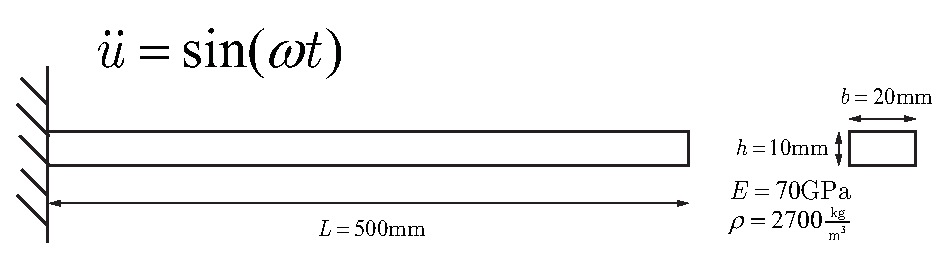
\includegraphics[width=0.6\textwidth]{fig/enunciado.eps}
	\caption{Se resolvió para una viga de aluminio empotrada excitada por una aceleración uniforme.}\label{fig:enunciado}
\end{figure}
Cabe destacar que el enunciado original otorgado por la cátedra sugería usar para la aceleración excitadora $\ddot{u}=\sin (\Omega x)$, el cual nos daría un sistema cuasiestático poco interesante.\footnote{a no ser que $\Omega$ esté en función del tiempo y no se haya especificado}

\subsection{Método}
Se resuelve el problema por método de los elementos finitos utilizando vigas de dos nodos. Cada nodo tiene dos grados de libertad, $v$ como el desplazamiento en $y$ y $\theta$ siendo el giro de la viga en el plano $x\!y$.

La matriz de masa usada es \textit{consistente}. Esta y la matriz de rigidez toman la forma: \cite[p.379]{cook2007concepts}
\[
\Mme{m}_{\mathrm{viga}}=\frac{\rho A L}{420}\left[\begin{array}{cccc} 156 & 22\,\mathrm{L} & 54 & -13\,\mathrm{L}\\ 22\,\mathrm{L} & 4\,{\mathrm{L}}^2 & 13\,\mathrm{L} & -3\,{\mathrm{L}}^2\\ 54 & 13\,\mathrm{L} & 156 & -22\,\mathrm{L}\\ -13\,\mathrm{L} & -3\,{\mathrm{L}}^2 & -22\,\mathrm{L} & 4\,{\mathrm{L}}^2 \end{array}\right] \qquad \qquad \Mme{k}_{\mathrm{viga}}=\frac{E I_z}{L^3} \left[\begin{array}{cccc} 12 & 6\,L & -12 & 6\,L\\ 6\,L & 4\,L^2 & -6\,L & 2\,L^2\\ -12 & -6\,L & 12 & -6\,L\\ 6\,L & 2\,L^2 & -6\,L & 4\,L^2 \end{array}\right]
\]

Se resuelve el problema de autovalores para el sistema sin amortiguamiento \eqref{eq:eigenvalueproblem} y se obtienen las frecuencias naturales del sistema 

\begin{equation} \label{eq:eigenvalueproblem}
	\left( \Mme{K} - \omega^2 \Mme{M}\right)\Cme{D}= 0
\end{equation}

Luego se busca la respuesta armónica del sistema ante la carga conocida 




\subsection{Resultados}
Las primeras tres frecuencias naturales obtenidas con una solución de 8 elementos.
\[
\Cme{\Omega} = \begin{Bmatrix}
\vdots \\
7259 \si{\, \radian \per \second}\\
2591 \si{\, \radian \per \second}\\
413 \si{\, \radian \per \second}
\end{Bmatrix}=\begin{Bmatrix}
\vdots \\
1155\, \textrm{hz}\\
412\, \textrm{hz}\\
65,8\, \textrm{hz} 
\end{Bmatrix}
\]


\begin{figure}[htb!]
	\centering
	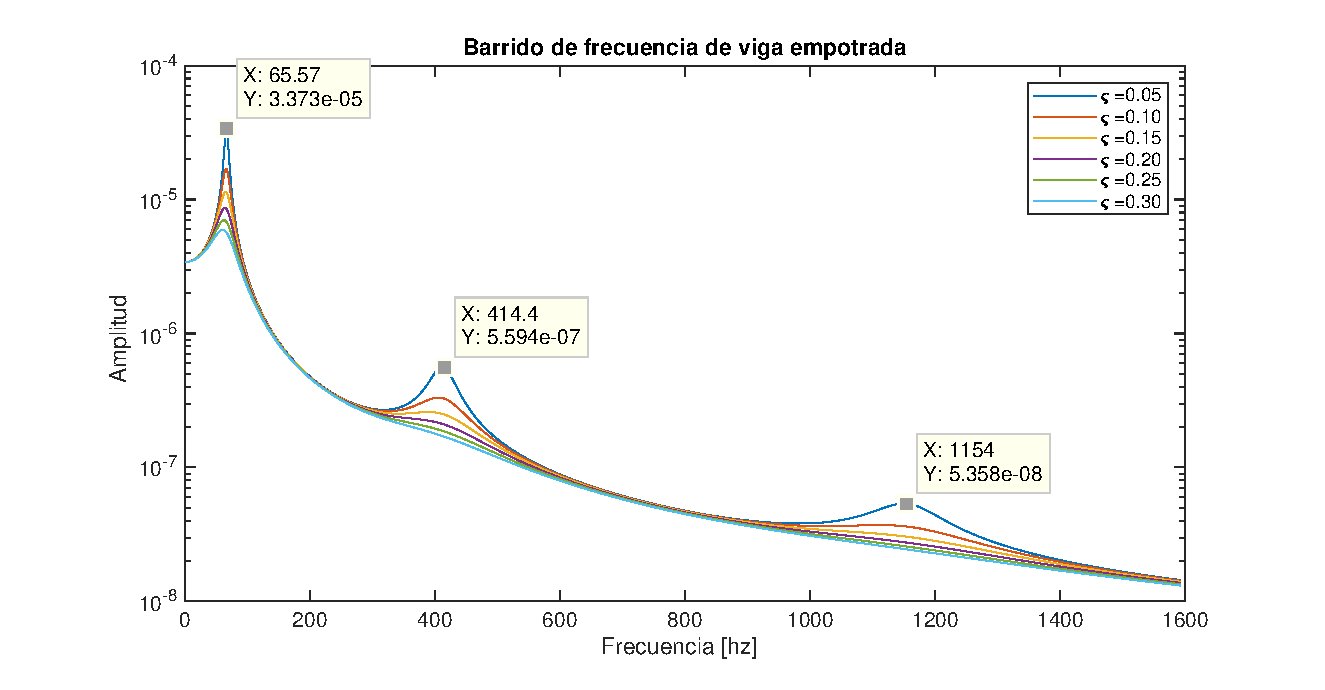
\includegraphics[width=0.8\textwidth]{fig/sinesweep.eps}
	\caption{Barrido de frecuencia \textbf{modal}. Valores de amplitud máxima recuadrados.}
\end{figure}

\begin{figure}[htb!]
	\centering
	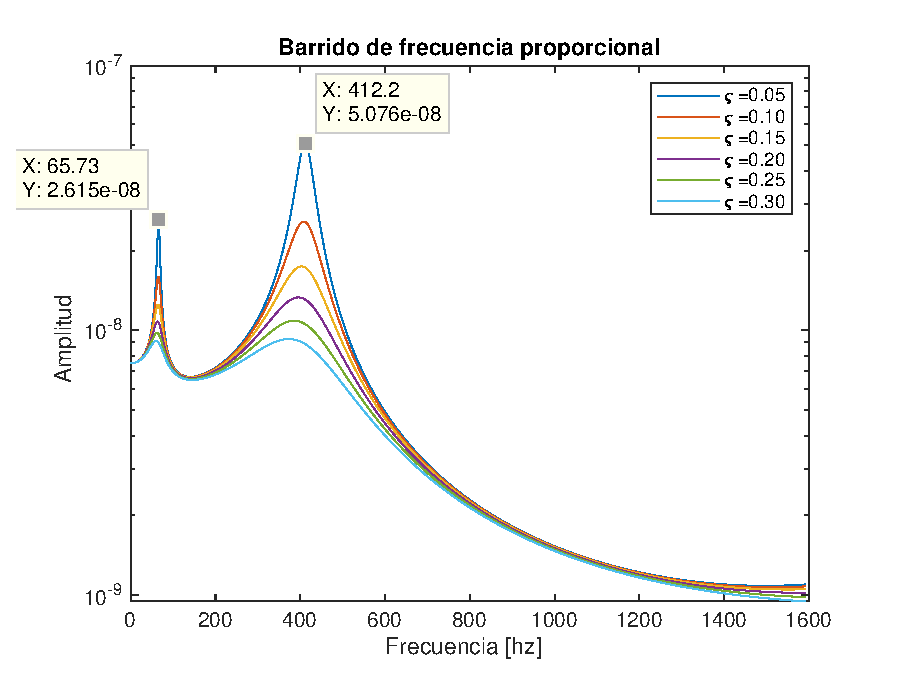
\includegraphics[width=0.8\textwidth]{fig/sinesweepprop.eps}
	\caption{Barrido de frecuencia \textbf{proporcional}. Valores de amplitud máxima recuadrados.}
\end{figure}


\subsection{Conclusiones}


\clearpage
\bibliography{labibliografia} % Indica archivo
\bibliographystyle{plainnat} 

\end{document}